\chapter{Background}
\label{ch:background}

\section{MathLang for Mathematics}
\label{sec:mathlangbackground}

\Gls{math} originally started in 2000. It's original goals was to allow gradual \gls{computerise} and \gls{formalise} of mathematical texts.

Maarek \cite{manuelphd} describes \gls{math} in the 3 following points:

\begin{enumerate}
\item \textit{MathLang is} \textbf{a framework.} It is meant to be used for communication as a concrete support for human mind formulation. MathLang is a well structured framework aimed to synthesize the common mathematical language.

\item \textit{MathLang is} \textbf{for mathematics}. It is meant to be open to any branch of mathematics and to any topic that uses mathematics as a base language. MathLang mimics mathematics in its incremental construction of a body of knowledge.

\item \textit{MathLang is} \textbf{for computerisation.} MathLang is meant to be a medium for a human-system, human-human via a digital support, and system-system communication. MathLang is a computer-based framework and therefore offers automation facilities.

\end{enumerate}

MathLang is not a system for proof verification but a framework to computerise and translate information (such as mathematical text) into a form on which proof checkers can operate.

The MathLang framework provides extra features supporting more rigour to translation of the common mathematical language. One can define further levels of translations into more semantically and logically complete versions. This gradual computerisation method should be more accessible than direct formalisation, because a number of first levels do nor require any particular expertise in formalisation.

So far Mathlang has given alternative and complete paths which transform mathematical texts into new computerised and formalised versions. Dividing the formalisation of mathematical texts into a number of different stages was first proposed by N.G. de Bruijn to relate common mathematical language to his Mathematical Vernacular \cite{mv} and his proof checking system Automath.

\subsection{The Current MathLang Design \label{sec:currentmath}}
The MathLang Framework instructs the computerisation process to be broken up into a number of levels called \textbf{aspects}. Each aspect can be worked out independently, simultaneously or sequentially without prior knowledge of another aspect. The current MathLang Framework contains three well-developed aspects, the \gls{cga}, the \gls{tsa} and the \gls{dra}, and has further aspects such as the Formal Proof Sketch.

\begin{figure}[H]
\begin{center}
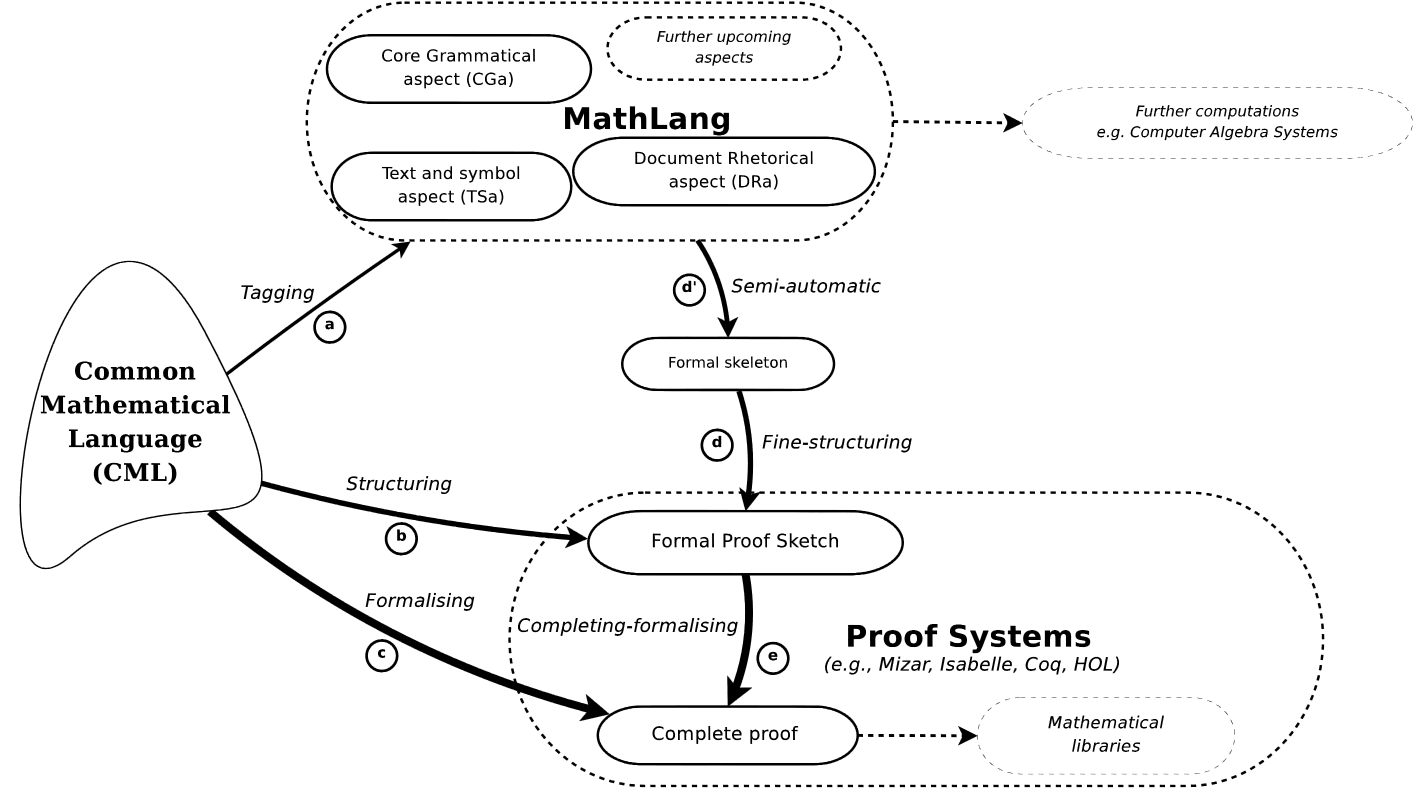
\includegraphics[scale=0.255]{Figures/Background/mathlang.png}
\end{center}
\caption{The MathLang approach to computerisation/formalisation \cite{mathintomizar}\label{fig:mathlang}}
\end{figure}

Figure \ref{fig:mathlang} shows the overall situation of work in the current MathLang Framework.
The labelled arrows show the computerisation paths from the common mathematical language to any proof system. The width of the arrow representing each path segment increases according to the expertise required. The level of expertise needed to computerise a CML text straight into a complete proof is very high, however the level of expertise is much smaller by using the \gls{math} framework to help form a formal skeleton and then into a complete proof. The dashed arrows illustrate further computerisation that one can envision.

\subsection{Core Grammatical aspect \label{subsec:cga}}
The current \gls{cga} in MathLang uses a finite set of grammatical \textit{categories} to identify the structure and common concepts used in mathematical texts. The aims of the \gls{cga} is to make explicit the grammatical role played by the elements of mathematical texts and to allow the validation of the grammatical and reasoning structure within the \gls{cga} encoding in a mathematical text. The \gls{cga} checks for grammatical correctness and finds errors like an identifier being used without and prior introduction or the wrong number of arguments being given to a function \cite{krzysztofphd}.

\subsection{Text and Symbol aspect \label{subsec:tsa}}
The \gls{tsa} builds the bridge between a mathematical text and its grammatical interpretation. The \gls{tsa} is a way of rewriting parts of the text so they have the same meaning. For example some mathematicians may prefer to write "a=b and b=c and c=d", others may prefer "a=b, b=c, c=d" and some others may prefer "a=b=c=d". As you can see all these methods of writing have the same meaning however some symbols are different. The \gls{tsa} annotates each expression in the text with a string of words or symbols which aim to act as the mathematical representation of which this expression is. This allows everything in the text to be uniform.

\subsection{Document Rhetorical aspect \label{subsec:dra}}

The Document Rhetorical aspects checks that the correctness of the reasoning in the mathematical document is correct and that there are no loops. The \gls{dra} mark-up system is simple and more concentrated on the narrative structure of the mathematical documents whereas other previous systems (such as DocBook \footnote{http://www.docbook.org}, Text Encoding Initiative \footnote{http://www.tei-c.org/index.xml}, OMDoc \footnote{http://www.omdoc.org}) were more concentrated on  the subtleties of the documents. It is used to describe and annotate chunks of texts according to their narrative role played within the document \cite{krzysztofphd}. Using the \gls{dra} annotation system we can capture the role that a chunk of text imposes on the rest of the document or on another chunk of text. This leads to generating dependency graphs which play an important role on mathematical knowledge representation. With these graphs, the reader can easily find their own way while reading the original text without the need to understand all of its subtleties. Processing \gls{dra} annotations can flag problems such as cicular reasoning and poorly-supported theorems.

\subsection{Full formalisation paths into Theorem Provers}

The MathLang project started in 2000 when F.Kamareddine and J.B. Wells started the project within Heriot-Watt University as part of the ULTRA group \cite{researchprop}. It was an idea for a new mathematical language and framework to keep most of the advantages of Common Mathematical Language (CML) and avoid it's disadvantages. This framework would allow a gradual computerisation and formalisation of mathematical texts.

The framework was first set out in 2003 \cite{firstyear} and then saw an established path for conversion of a mathematical text written in CML into the isabelle proof assistant using rules and MathLang annotations \cite{secondyear}. A few short projects (by 4th year undergraduate dissertations or MSc students) have developed MathLang into the Framework it is today. A prototype of the Core Grammatical aspect and Text and Symbol aspect were defined in the PhD thesis of Manuel Maarek \cite{manuelphd} and then a gradual computerisation into the Mizar proof assistant using the three key aspects of MathLang were a great success and published \cite{mathintomizar}.

The design of the \gls{cga} is due to Kamareddine, Maarek and Wells \cite{oomathlang} and the implementation of the \gls{cga} is due to Maarek \cite{manuelphd}. The design of the \gls{tsa} is due to Kamareddine, Maarek, and Wells with contributions by Lamar to the souring rules \cite{restoringtsa}, \cite{manuelphd}, and \cite{lamarphd}. The implementation is primarily by Maarek \cite{manuelphd} with contributions from Lamar \cite{lamarphd}. The design and implementation of \gls{dra} were the subject of Retel's thesis \cite{krzysztofphd}. Further additions have since been carried out by Zengler \cite{cmtim}.

\subsection{Conclusion}
A lot of work has already been completed on the MathLang Framework. The three aspects, \gls{cga}, \gls{dra}, and \gls{tsa}, have been designed and redesigned so that a variety of mathematical texts and symbols could be used. Then the aspects have been implemented for ease of access. A translation from a mathematical text into the Mizar proof checker has been worked through and described in detail in a published paper \cite{mathintomizar} and a PhD thesis \cite{manuelphd}. A partial translation from a CML text into the Isabelle Syntax has also been carefully described in the 2009 paper \cite{mathintoisa} and also written in a PhD thesis \cite{lamarphd}. Some of the future work described was to allow MathLang to be used as a tool to computerise other pieces of information, such as another piece of academic text yet it does not need to be mathematical.

\section{Formal Methods in practice}
\label{sec:formnot}

Formal methods are mathematical approaches to software and system development which support the rigorous specification, design and verification of computer systems \cite{fmeurope}. Specifications are a collection of statements describing how a proposed system should act and function. Formal specifications use notations with defined mathematical meanings to describe systems with precision and no ambiguity. The properties of these specifications can then be worked out with more confidence and can be described to the customers and other stakeholders. This can uncover bugs in the stated requirements which may not have found in a natural language specification. With this, a more complete requirements validation can take place earlier in the development life-cycle and thus save costs and time of the overall project. The rigor using formal methods eliminates design errors earlier and results in substantially redecued time \cite{benefitsofform}. 

Abrial presents two case studies in \cite{10.1145/1134285.1134406} describing the use of formal methods in industry. He concludes that one of the problems is that some managers are afraid that engineers will not be able to perform the interactive proofs. This thesis proposes to address this problem by inventing a method for a thereom proving novice to translate a formal specification into the theorem prover with little or no knowledge of the chosen theorem prover. The research presented here proposes to provide an addition to testing and not a replacement. However the effort and costs should be reduced in the testing stages as the bugs would be found earlier in the specification and verification phase of the project. As well as giving the proposed system a highier level of rigor.

\subsection{The use of Formal Methods in Industry}

Despite these advantages some managers sometimes argue the cost of producing a system using formal methods do not cover the costs. However the rigour using formal methods eliminates design errors earlier and results in substantially reduced time. Investing more effort in specifying, verifying and testing will benefit software projects by reducing maintenance costs, higher software reliability and more user-responsive software \cite{chantatub}.

Even in the 21st century we still experience a `software crisis' where software projects are being delivered far behind schedule, quality is poor and maintenance is expensive. This software crisis allows for bad software to be released e.g. the computer system `Sabre' \cite{sabre}, which went off-line for almost a day leading to the cancellation of more then 700 flights.

Well engineered software is software which is suitable, efficient, reliable and maintainable with low costs and on schedule.

The cost of testing is around 50\% of the entire project cost. Maintenance cost is 2-4 times greater than pre-delivery cost. In large projects, failure to find and correct software errors can increase the cost of the software by 100 times, in small software projects it's usually about 2-4 times more \cite{andrewslides}.
Therefore more effort should be spent in requirements analysis and design to catch errors early in the project life-cycle. The \gls{computerise} of formal specifications using the MathLang framework should help with requirements analysis, as it is concentrating more on getting the requirement specifications correct and thus minimising errors later on in the project life cycle. For example, in the Sholis project \cite{sholis}, using a formal specification was most effective for fault finding, therefore if the specifications are correct, then the program implemented should then in turn contain less errors if it follows the correct specification.

King, Hammond, Chapman and Pryor's paper \cite{sholis} was based on the SHOLIS defence system. It highlighted the importance of having a formal specification on a system to check for errors. It was found that the Z proof was the most cost effective for fault finding. The Z specification found 75\% of the total faults for the system. Since Z specifications are important for finding faults in SIL4 systems (based on the sholis project), then checking the correctness of the Z specification is itself very important. Note that the specifications found 75\% of errors and not 100\%. As human error can still occur in formal specifications, using the ZMathLang approach may increase the percentage of errors found.

Hehner \cite{hehner99} also supports the use of specifications. He states it is the job of the specification to distinguish those things that are desirable in the program however when looking through a specification just with the human eye \cite{sholis} it is easy to make errors. Which is why checking the correctness of a specification through a theorem prover would help.

One reason industry may be reluctant to use formal methods is because they might perceive that the methods are too complicated for the benefits gained. Simplifying these formal methods so that anyone could understand may pose a great benefit and thus may be used more often in industry.

Hehner questions if all programs should have specifications. Which leads to the question of should simple programs also have specifications as well as high integrity systems. The benefits of planning and specifying a program far outweigh the time and cost of catching bugs and errors at a later stage \cite{planning} of complex programs. However it may be too time consuming for smaller program and it would be up to industry leaders themselves to decide.

Specifications, Programs, and Total Correctness \cite{hehner99} outlines that a programming language should not be the specification language. As not all industry experts are programming experts, the specification should be open for everyone in the team to understand the program not just the developers.

Hehner also states that \gls{total} is a mistake and \gls{partial} is enough. This may be because some software such as on aircraft's need to be running all the time when in the air and do not need to terminate. However with other programs it is important that they do terminate as a safety feature for example the automatic track gauge changeover for trains \cite{automatictrain}. It is important that the program should terminate if anything should happen such as errors or a crash, therefore \gls{total} of only some programs is needed.

An Introduction to Proving the Correctness of Programs \cite{hantler} describes the specification of correct behaviour of a program by the use of input/output assertions. This would be very expensive in very large programs. So it may be good for smaller programs only. Assertion is a very basic approach.

However with this approach, checking for correctness can only be done by an expert in that particular programming language. They will have to understand where a procedure starts and where a procedure ends. By checking the correctness of specifications using the ZMathLang method it will allow for many program specifications to be checked by a wider audience and not just expert programmers.

The assumptions used in the example on page 336 \cite{hantler} resulted from an unresolved execution of the IF statement.

A paper reflecting on industry experience with proving properties in SPARK \ref{DBLP:conf/itp/ChapmanS14}, describes a programming language and verification system that will offer sound verification for programs. It states that SPARK and the use of proof tools remain a challange (published in 2014) as the `adoption hurdle' is percieved too high. Customers and regulators have taken a variety of stances on static analys and theorem provers. Where some places in industry have adopted the idea others remain sceptical. Hopefully this thesis will present an idea on how formal analysys could be simplified and broken up into smaller more understandable steps and thus would allow more users to take on the idea.

\section{Methods for checking for Software Correctness}

Traditionally, functional correctness has been obtained with pen and paper or an interactive proof assistant. Well-designed program verifiers are reducing the effort involved in doing full verifications.

Proof assistants sometimes limit which program properties they reason about. By using the \gls{zmath} framework the specification would undergo different levels of rigor (and thus different types of checks) for example one might only want to check the grammatical correctness of the specification or one might want to fully formally prove the specification, different projects require different amounts of verification therefore the \gls{zmath} will allow this choice.

Dafny \cite{dafny} features modular verification, so that the separate verification of each part of the program implies the correctness of the whole program. This is similar to \gls{zmath}, where Dafny checks different parts of the text and thus confirms correctness of the full text, \gls{zmath} checks the correctness of the text through different levels of rigor to imply and fully correct specification.

Dafny was able to do a proof for the Schorr-Waited Algorithm, however the writer states that the loop invariants are complicated because they are concrete. A refinement approach such as Jean-Raymond Abrials \cite{abrial} may be preferred in this case.  

Another attempt at checking for correctness was written by Rex L.Page in Engineering Software Correctness \cite{engineeringsoftwarecorrectness}. A general theme within this paper, is that design and quality are important in engineering education. When teaching students how to create programs, it is not enough just to teach them how to develop software but to how develop good quality software. This paper describes experiments with the use of ACL2 (a subset of lisp), which is embedded on mechanical logic to focus on design and correctness. Using ACL2 emphasises the importance of software design and correctness. 

ALC2 is coded therefore users must know how to code software to formulate proofs. The intention of \gls{zmath} is to allow many people in the development team to be able to formulate proofs such as project managers, designers, engineers etc. Therefore no coding is neccessary and no new programming language is needed.

PVS (Prototype Verification System) \cite{pvs} is an environment for constructing specifications and developing proofs which have been mechanically verified. PVS has it's own specification language, which engineers would need to learn as well as using the environment for proofs. Type checking is undecidable for the PVS type system. The PVS also provides a language for defining high-level inference strategies.

Another tool which analysis the Z notation is Hol-Z \cite{hol-z}, which is also a proof environment for Z. Hol-Z is embedded in Isabelle/HOL therefore it provides a Z type checker, documentation facilities and refinement proofs with a theorem prover. The Z specification is implemented in \LaTeX{} then typed checked using an external plug in Zeta, it is then transformed into SML files to be added into the Hol-Z theorem prover environment. The user will need to have some good expertise in using the Hol-Z proof environment in order to fully prove the specification.

Fuzz \cite{spiveyfuzz} is another example of a typechecker for the Z language. It includes style files for \LaTeX{} and checks for the logical correctness and Z type correctness of Z specifications. This is different to the \gls{zcga} type checker as the weak types in \gls{zcga} check for the grammatical correctness and not the full logical correctness of Z. Therefore the grammatical correctness of partially formal specification can aslo be checked. The \gls{zmath} framework presented in this thesis uses the `zed' \LaTeX{} style package to typeset the Z specifications in the documents.

There are many other tools for Z which can be found on the Z Notation Wikia page \cite{zwikia}. For this thesis we will concentrate on translating Z specifications into theorem prover Isabelle \cite{isabelle}. Isabelle is a generic proof assistant which allows mathematical formulas to be expressed in a formal language and includes numerous contributions worldwide. It contains a large mathematical toolkit (majority of Z can be represented in Isabelle) and has a lot of support in forms of documentation and online. It is distributed for free, easy to find, download and install and is regularly updated. The original \gls{math} has translated mathematical texts into Isabelle already (\cite{mathintoisa}) therefore we can use parts of that research to aid the research in this thesis.

\section{Proof carrying-code}

\Gls{pcc} is a framework for the mechanical verification of safety properties in machine language programs. The provider of the \gls{pcc} must provide both the executable code and a machine-checkable proof. This is to ensure the safety of the executable code so that it doesn't access any other data it is supposed to. Appel \cite{fpcc} attempts to make \gls{pcc} easier by using foundational method where he avoids any commitment to a particular type system or a verification checker. \gls{zmath} uses a similar approach as the specification goes through different types of correctness checks and only at the very end, picks a verification checker to translate into. All the steps until the final three (see figure \ref{fig:steps}) do not require the user to commit to a particular theorem prover.

\Gls{pcc} has several characteristics that allow it to execute foreign code safely. A critical components of any \gls{pcc} implementation is the safety policy which is specified at the start, before any implementation takes place. This policy uses safety rules that the consumer of the machine code desires for any untrusted code. \Gls{pcc} is a two stage verification process \cite{suappc}, using a `proof producer' and a `code consumer' to do the work. The proof producer must produce two kinds of work, one is the machine code and the other is the proof to verify that the machine code is safely executable. \Gls{pcc} is slightly different to \gls{zmath} as \gls{pcc} includes the proof with the code of the program. Since a large system may have lots of different components which join to make one large system. The proof carrying code would need to be implemented in all of the components (or the most safety-dependent) components. Formal specifications can display and abstract view of the entire system and it's individual components. Therefore the entire system as a whole could be checked. However added rigor, one can use the \gls{zmath} framework to check the correctness as a whole system and then using proof carrying code to check the code itself for correctness.

Manish Mahajan \cite{pccman} explains that any implementation of \gls{pcc} must contain at least 4 elements: (1) formal specification language used to express the safety policy, (2) a formal semantics of the language used by the untrusted code, (3) a language used to express the proofs and (4) an algorithm for validating proofs. \Gls{zmath}'s \gls{dra} and \gls{cga} could be useful in creating and checking the formal specification needed to express the safety policy, (1), which again could add a level of rigor to the system. Mahajan also writes that the size of binary will be increased due to inclusion of the safety proof, this safety proof can be done during the formal specification part of the project, thus minimizing the size of the safety proof needed for the \gls{pcc}.

\section{Z Syntax and Semantics}

The Z notation is based on set theory and mathematical logic. It is a particular formal method which was developed to specify the new Customer Information Control System (CICS) functionality \cite{cics}. The set theory includes standard set operators, set comprehensions, cartesian products and power sets. Z also has other aspects such as schemas which are used to group mathematical objects and their properties. The schema language can be used to describe the state of a system and ways in which that state may change \cite{Woodcock:1996:UZS:235337}.

In the Z notation there are two languages: the mathmatical language and the schema language. The mathematical language is used to describe various aspects of a design: object, and the relationships between them. The schema language is used to structure and compose descriptions: collecting pieces of information and naming them for re-use. A schema consists of two parts: a \emph{declaration part} and a \emph{predicate part}. The \emph{declaration part} consists of declared variables and the \emph{predicate part} describes the variable values. We can write a schema either horizontally (figure \ref{fig:horizontalschema}) or vertically (figure \ref{fig:verticalschema}).

\begin{figure}[H]
\vspace{-0.2in}
\centering
\begin{minipage}{0.45\textwidth}
\begin{zed}
\noindent Schema\ Name \defs [declarations | predicates]
\end{zed}
\vspace{-0.18in}
\caption{An example of a schema written horizontally.\label{fig:horizontalschema}}
\vspace{-0.2in}
\end{minipage}\hfill
\begin{minipage}{0.45\textwidth}
\begin{schema}{Schema\ Name}
declarations
\where
predicates
\end{schema}
\vspace{-0.2in}
\caption{An example of a schema written vertically. \label{fig:verticalschema}}
\vspace{-0.2in}
\end{minipage}
\end{figure}

If we wanted a property of some system which consists of two variables $x$ and $y$ and state that $x$ must be smaller than $y$ then we can write:

\begin{schema}{xLessThany}
x: \nat \\
y: \nat
\where
x < y
\end{schema}

The full language of Z can be explored in \cite{spiveyreferencemanual}, \cite{essenceofz} and \cite{Woodcock:1996:UZS:235337}.

The semantics of Z has helped in the design of better specification languages by allowing critical comparisons of specification techniques. The semantics of Z \cite{formsem} gives us a head start in formulating the different aspects of \gls{zmath}. The study in the semantics of Z provide a foundation for reasoning about specifications.

In \cite{formsem} it states that many of the proofs needed during the development process are `\textit{very shallow but contain a mass of detail}'. This detail may be difficult to understand by some stakeholders or team members in the system design team. \Gls{zmath} would aid in this as it is a tool which produces documents which anyone in the development team/clients would be able to understand.

The paper also states that \textit{consistency, completeness and refinement are essential to program development}. Therefore if the specification is consistent, complete and refined then the program will be as well (as long as the program sticks to the specification). Which makes it very important to have the specification checked as well as the program for errors. Spivey also says that `\textit{theory  of signatures is decidable and therefore well suited to mechanical checking using a proof checker such as Mizar or Coq}'. However Mizar and Coq usually requires a lot of expert level knowledge to prove the specification directly. Therefore a major aim of this thesis is to develop a path to break up the translation into a theorem prover such as Isabelle, Coq or Mizar.

This thesis uses a lot of the specifications in Ed Currie's book, An Essence of Z \cite{essenceofz}. The book would be a beneficial text to check for correctness as it is used in academia to teach students Z. The framework developed in this thesis is for novices to get to grips with checking the correctness of Z specification and translating them into a theorem prover. It does not promise to turn novices into theorem prover experts overnight but give them a guide with verifying the correctness of specifications. The research presented here is also not intended for theorem prover experts however users who are experts in theorem proving may also find some steps of the \gls{zmath} framework beneficial such as the \gls{zcga} or \gls{zdra}. The Essence of Z is also starts with very basics of logic to larger specifications which can be used a real software systems. It contains more then one specification and therefore gives a variety of syntax to use the \gls{zmath} framework on.

\section{Types and their desirable properties}

Type systems are good for many things \cite{pierce}, one of which includes that it allows early detection of some programming errors. Errors that are detected early can be fixed straight away rather then it lingering around to be discovered much later. Errors can often be pinpointed more accurately during type checking more often then in run-time, when their effects may not become visible until after some things go wrong, which in high integrity systems can have disastrous results. Type systems support the programming process by enforcing disciplined programming. Type system form the backbone of the module languages used to packaged and tie together all the different parts of large scale software systems. Types are also useful when reading programs. They form a useful documentation to the reader about the behaviour of the program, this form of documentation can not be outdated like comments since when the program specification changes so does the types involved.

Type-free lambda calculus \cite{bar93} allows for every expression to be applied to every other expression, eg I = $\lambda x.x$ may be applied to any argument $x$ to give the same result $x$. The expression may also be applied to itself. There are also typed versions of lambda calculus introduced by Curry \cite{cu34}. Types are usually objects of a syntactic nature and may be assigned to lambda terms. Using Types in this nature, this thesis describes a way in the \gls{zcga} (chapter \ref{ch:zcga}) assigns grammatical types to parts of a specification written in Z or partially written in Z. By doing so, the grammatical correctness of a system specification could be checked. The grammatical types are an adaptation from the grammatical categories taken from \cite{wtt}. One of the main benefits of the \gls{zcga} is it can check the grammatical correctness of partial formal specifications, that is specifications which are written in natural language and are on the way to becoming formal. Other Z type checkers such as Z/Eves \cite{Saaltink99thez/eves} and Fuzz \cite{spiveyfuzz} check the logical type correctness of a fully formalised Z specification.

\section{Generating properties to prove for Formal Specifications}

\begin{defin}
A logical formula associated to a correctness claim for a given verification property. The formula is valid if and only if the property holds. The correctness of the property under verification is “delegated” to proving the correctness of the new formula \cite{handbookofembed}.
\end{defin}

Therefore a proof obligation is a logical formular which the specifier must show to be a consequence of the specification so that a specification can be taken to be acceptable. In a more pragmatic sense proof obligations may be viewed as what the developer of a specification is obliged to prove in order to confirm that development is consistant.

Woodcock and Cavalcanti \cite{woodcock2004tutorial} use the alphabetised relational calculus to give denotational sematics to different constructs from programming patterns. This paper describes `\emph{healthiness conditions}' which identifies properties that characterise theries. Each one of these healthiness conditions represents a fact about the computational model for the programs being studied.

\begin{exam}
The variable `\emph{clock}' is an observation of the current time which is always moving onwards. The following predicate `B' specifies the clock variable:

\begin{zed}
B \defs clock \leq clock'
\end{zed}
\end{exam}

The healthiness condition described in this paper are specific proof obligations for the concept of \gls{utp}. The semantic model of \gls{utp} is presented a Z specification. Therefore the healthiness conditions for the specification would in one way be checking for the correctness of the \gls{utp} model. In a similar way, it is important to add healthiness conditions or as we call them in this thesis, `safety properties' in order to check each individual specification for various types of correctness.

Stepney describes two proof project written in Z in her paper a tale of two proofs \cite{stepney1998tale}. She explains how the proof process is deelply affected by \textbf{why} something is being proved, \textbf{what} is being proved and \textbf{how} the finished proof is to be presented. Stepney suggests that the proofs for specifications themselves do not have to be deep but the workings of what to proves can add to the labour. It is also important to keep in mind how deep the customer wants the proof and what level of assurance they need. She highlights 5 different points to prove:

\begin{figure}[H]
\begin{enumerate}
\item \textbf{Consistency checks}: Prove that your specification is cosistent and that it has a model.

\item \textbf{Sanity Checks}: In a `state and operations' style specification, prove that the state invariants are satisfied throughout and that the precondition of each operation is not \emph{false}.

\item \textbf{Emergent properties of a single specification}: Make explicit as a theorem some desired or suspected property of the specification, then prove it holds.

\item \textbf{Required properties of a single specification}: If some property is required to hold of the specification, and the specification has captured it implicitly, it needs to be made explicit and shown to hold.

\item \textbf{Properties across specifications}: Prove that a certain relationship holds between two specification such as the refinement relationship.
\end{enumerate}
\caption{Different points to prove in a specification \cite{stepney1998tale}. \label{fig:ptp}}
\end{figure}

Some of the points in figure \ref{fig:ptp} would be fairly easy to automate such as `consistancy checks' and `santity checks' however the other 3 points would be difficult to automate as they would all depend on the specification in question and would perhaps need some \emph{extra information} to decipher these properties. For example if one wish to automate proof obligations from point 5 the user would need to implement another specification (such as a refinement specification) and then prove the relationship between the original specification and the new one. In this thesis, we will concentrate on properties described in point 1 which have been automated. 

Stepney also explains that if the development process is incremental, it would be worthwhile getting a good structure for a proof up front which you can add more details in later. \gls{zmath}  can automatically generate this first structure which could be added to if needed. It can produce a specification in Isabelle syntax where other properties and details could be added to by the user at a later stage.

Most recently Mark Adams \cite{JFR4576} describes that even formalisation itself can be prone to error and therefore even if we do get a fully proven specification, the proof will also need to be checked. He outlines the flyspeck project which assists with the checking of formalised proofs. Adam calls this `\emph{proof auditing}', which adds another step of rigour to the theorem. \gls{zmath} assists with translating the specification into a theorem prover along with consistancy lemmas to prove. The user can then choose to prove these lemmas and the proof audit their thereom. However, even if proof auditting adds another level of rigour it is important to keep in mind who the user is doing the proofs for. As Stepney pointed out in \cite{stepney1998tale}, some clients wouldn't need that amount of rigor for their projects and only the proved safety properties may be enough.

Woodcock et al also describes that a specification can be developed in such a way that can lead to a suitable implementation called refinement \cite{Woodcock:1996:UZS:235337}. 

To refine a formal specification, more data must be added e.g. how certin calculations should be carried out. He states an abstract specification may leave design choices unresolved and its up to the refinement specificatino to resolve some of these choices. An example of this is shown in the following:

\begin{exam}

\begin{schema}{ResourceManager}
free: \mathbb{F} \nat
\end{schema}

 Any resource that is free can be allocated

\begin{schema}{Allocate}
\Delta ResourceManager \\
r!: \nat
\where
r! \in free \land free' = free \setminus \{r!\}
\end{schema}

\label{exam:allocate} 
\end{exam}

If there is more than one resource free in example \ref{exam:allocate} then this will class the specification as non deterministic.

Example \ref{exam:allocate} can be refined in that if there is more than one resource free, the resource with the lowest number should be allocated. This is shown in the following example:

\begin{exam}

\begin{schema}{Allocate}
\Delta ResourceManager \\
r!: \nat
\where
r! \in min~free \land free' = free \setminus \{r!\}
\end{schema}
\label{exam:allocaterefine} 
\end{exam}

Refining an abstract specification which is descibed in \cite{Woodcock:1996:UZS:235337} and in \cite{spiveyreferencemanual} is exactly what Stepney points out in point 5 from figure \ref{fig:ptp}. To show that this property holds the user would need to produce another specification which refines their original one and then include propertie of how they relate to eachoether. Since each individual specification is different then refinement specifications would be different to. Thus we wouldn't be able to automate this point. \gls{zmath} aims to assist the user in translating and proving their specification, the proof effort will be focused on properties which can be automated e.g. item 1 in figure \ref{fig:ptp}. Items 3, 4 and 5 would be to difficult to automate and therefore out of the scope of this thesis.

Fraser and Banach \cite{DBLP:conf/sefm/FraserB07} state that model based formal methods usually come in the form of many incompatible tools. Therefore they devised a system to combine different techniques called the frog toolkit.

Many verification tools today tend to utilize a single technique and are unable to ineract easily with other tools in other kits. A more dynamic approach such as RODIN \cite{Jones05j} and Overture \cite{overture} are persuing a more flexible approach. \gls{zmath} will need to follow in the footstep of these two toolkits in order to be succesfull and not commit to a particular system until needed. This is why the steps 1-3 of the translation path (figure \ref{fig:steps}) are generic and can be used to translate the specification in any theorem prover. It is only at step 4 which is where we start committing to Isabelle.

The main aim of the frog toolkit was to support retrenchment, which is a formal technique used along side refinement. The new toolkit was created which was able to use a variety of techniques in a single working environment. The frog toolkit can prove the relationshipis between multiple specifications (which we see as point 5 in figure \ref{fig:ptp} from Stepney \cite{stepney1998tale}). To do this the user should have at least 2 specifications implemented to prove the relations (usually one is a refinement specification of the first one). These specifications where then written in frog-ccc, a meta language to use within the frog toolkit. \gls{zmath}'s aim is to prove the properties described as point 1 in figure \ref{fig:ptp} therefore another specification to refine the abstract one is not needed.

Since formal specifications are not executable it is difficult to verify the consistency of the specification. Wen, Miao and Zeng \cite{DBLP:conf/icsea/WenMZ06} present and approach to generate proof obligations to check for consistancy of object Z specifications. Checking for consistancy of specifications is described in point 2 in figure \ref{fig:ptp}. In their paper, the authors explain two 
types of proof obligations which check that a object Z specification is non conflictive. They are:

\begin{itemize}
\item Existence of initial state

\item Feasibility of an operation
\end{itemize}

The initial state is a state within the state space of the specification which should exist and satisfy the stateInvariants. In all specifications their should exist a state which initialised the beginning state of the specification.

An operation can tranform one state to another. Therefore if the operation is feasible, the pre state (state before the state change) and post state (state after the state change) should always satisfy the state invariant. 

We will use the definitions shown in \cite{DBLP:conf/icsea/WenMZ06} to automatically generate the proof obligations to check for the correctness of our Z specifications as the specifications we use in this thesis are all state based.

In summary there are many different approaches to finding properties to prove about formal specifications. Some which can be easily automated, some which need some more information and some which will need to be written manually. Since we do not expect the users of \gls{zmath} to be experts in the fields of theorem proving we want to attempt to automate proof obligations which can be easily understood by the user. Then once the user gains some knowledge of their theorem prover, they can add other proof obligations manually. As explained in this section, it is important to note who the user is doing the proofs for, as the customer may not need or want complex proofs. Therefore we shall generate the proof obligations which can be automated and do not require any extra information to be automated.

\section{Conclusion}
This chapter has described in depth the reasearch old and new which has relevence to this thesis. The MathLang framework which was designed and implemented for mathematics has been described and gives details of the method in which plain mathematical documents are formalised and translated into theorem provers. In this section we show a diagram which was proposed to identlify the steps in which a complete proof can be achieved from a mathematical text. 

The next section of this chapter highlights formal methods and formal languages used in practice. Formal methods which have been used in an industrial setting has been explained and analysed. We then outlined other methods for checking for software correctness which may or may not have been used in practice but also investigated in an academic setting.

Since this thesis concentrates on Z specifications we have outlined what are Z specifications and compared it with other formal languages. 

We also researched into types and their properties since the first aspect of \gls{zmath} is heavily based on a weak typing system.

This chapter concluded with different ways one can generate properties to prove their formal specifications.